\chapter{Численные результаты} \label{ch:ch3}
Применение сеточной адаптации с использованием методики погруженных границ рассматривалось на примере решения двумерной модельной задачи – численного моделирования течения вокруг цилиндрического препятствия при его движении справа налево с дозвуковой скоростью $U_B$ , соответствующей числу Маха равному 0.2. Число Рейнольдса Re рассчитанное по диаметру и скорости движения цилиндра полагалась равным 200. При численном решении данной задачи в качестве характерной скорости выбиралась скорость звука в невозмущенном потоке газа при нормальных условиях. Безразмерный радиус цилиндра $R$  устанавливался равным величине 0.2. Тогда эффективное числа Рейнольдса  Re при котором проводились расчёты имело значение 400.
\begin{figure}
	{\centering
		\subbottom[List-of-Figures entry][зона движения цилиндра\label{fig:setka1_a}]{%
			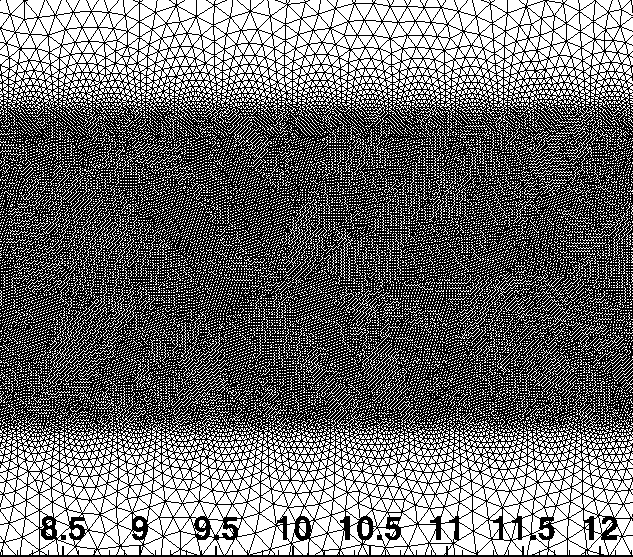
\includegraphics[width=0.45\linewidth]{figure1a}}
		\hfill
		\subbottom[окрестность препятствия\label{fig:setka1_b}]{%
			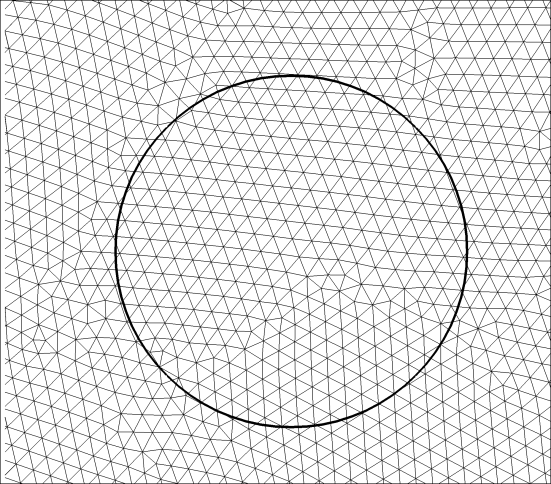
\includegraphics[width=0.45\linewidth]{figure1b}}
	}
	\caption[Фрагменты расчётной подробной сетки 1]{Фрагменты расчётной подробной сетки 1: (a) зона движения цилиндра, (б) окрестность препятствия.}
	\label{fig:setka1}
\end{figure}
\begin{figure}
	{\centering
		\subbottom[List-of-Figures entry][зона движения цилиндра\label{fig:setka2_a}]{%
			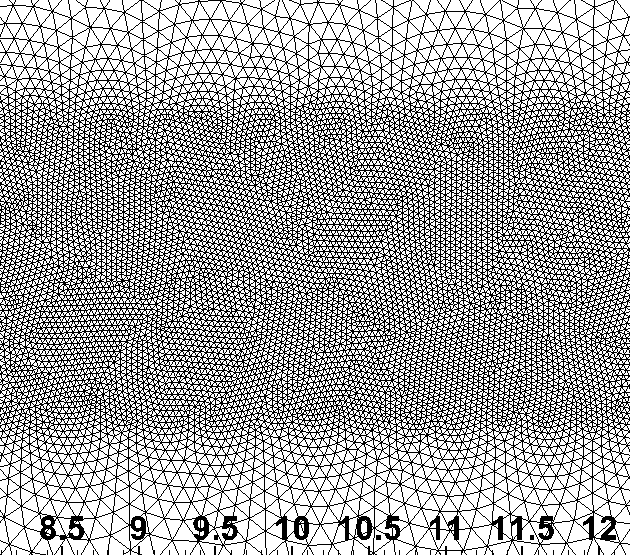
\includegraphics[width=0.45\linewidth]{figure2a}}
		\hfill
		\subbottom[окрестность препятствия\label{fig:setka2_b}]{%
			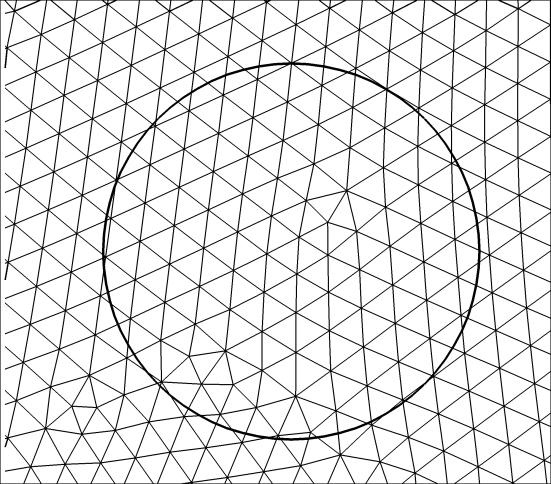
\includegraphics[width=0.45\linewidth]{figure2b}}
	}
	\caption[Фрагменты расчётной подробной сетки 2]{Фрагменты расчётной подробной сетки 2: (a) зона движения цилиндра, (б) окрестность препятствия.}
		\label{fig:setka2}
\end{figure}

Для проведения расчёта движения цилиндра необходимо иметь подробную сетку на всём пути движения цилиндра, во-первых, для корректного описания физических процессов, происходящих при обтекании препятствия, и во-вторых, для более точного описания границы обтекаемого препятствия при использовании метода погруженных границ. Поэтому использование неподвижных (неадаптивных сеток) приводит к резкому возрастанию вычислительной сложности решения такого типа задач. Применение адаптивной сетки, сгущающейся к границе движущегося тела, и обеспечивающее нужное разрешение сетки в следе за телом, должно уменьшить размер сетки, и, как следствие вычислительную стоимость решения. Таким образом, необходимо сравнить качество численного решения, полученного на трёх сетках – подробной, грубой и грубой с адаптацией.

Для этого расчёты проводились на трёх неструктурированных треугольных сетках. Первая сетка (сетка 1) – подробная сетка с числом узлов равным 391628 (рисунок~\ref{fig:setka1}), вторая сетка (сетка 2) – сетка с числом узлов 110372, приблизительно в 3.5 раза меньшим, чем у подробной сетки (рисунок~\ref{fig:setka2}).  Заметим, что в области движения цилиндра для сеток 1 и 2 определён регион квазиравномерной сетки с шагом $h$\footnote{ Квазиравномерная треугольная сетка — сетка, состоящая из равносторонних треугольников с длиной стороны равной $h$.} и от него происходит огрубление сетки к границам расчётной области (см. рисунках~\ref{fig:setka1_a}~и~\ref{fig:setka2_a})
Третья сетка (сетка 3) это сетка 2 адаптирующаяся к поверхности движущегося цилиндрического препятствия и не меняющая своей топологии. На рисунках~\ref{fig:setka3_mov}~и~\ref{fig:setka3_zoom} показаны фрагменты адаптивной сетки на различные моменты времени и положения движущегося цилиндра.
\begin{figure}
	{\centering
		\subbottom[List-of-Figures entry][начало периода $t_0$\label{fig:setka3_mov_a}]{%
			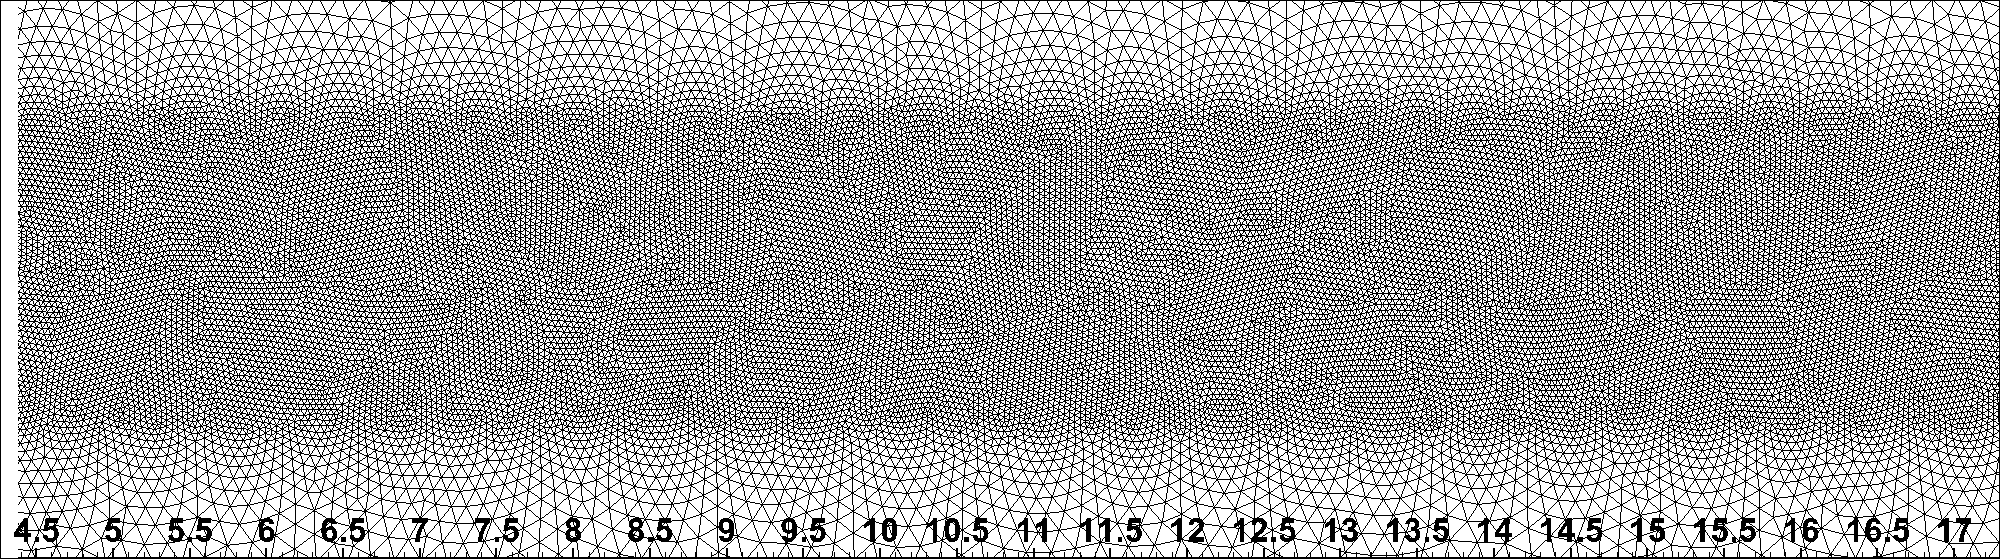
\includegraphics[width=0.9\linewidth]{figure3a}}\\
		\subbottom[полтора периода $t_0+1.5T$\label{fig:setka3_mov_b}]{%
			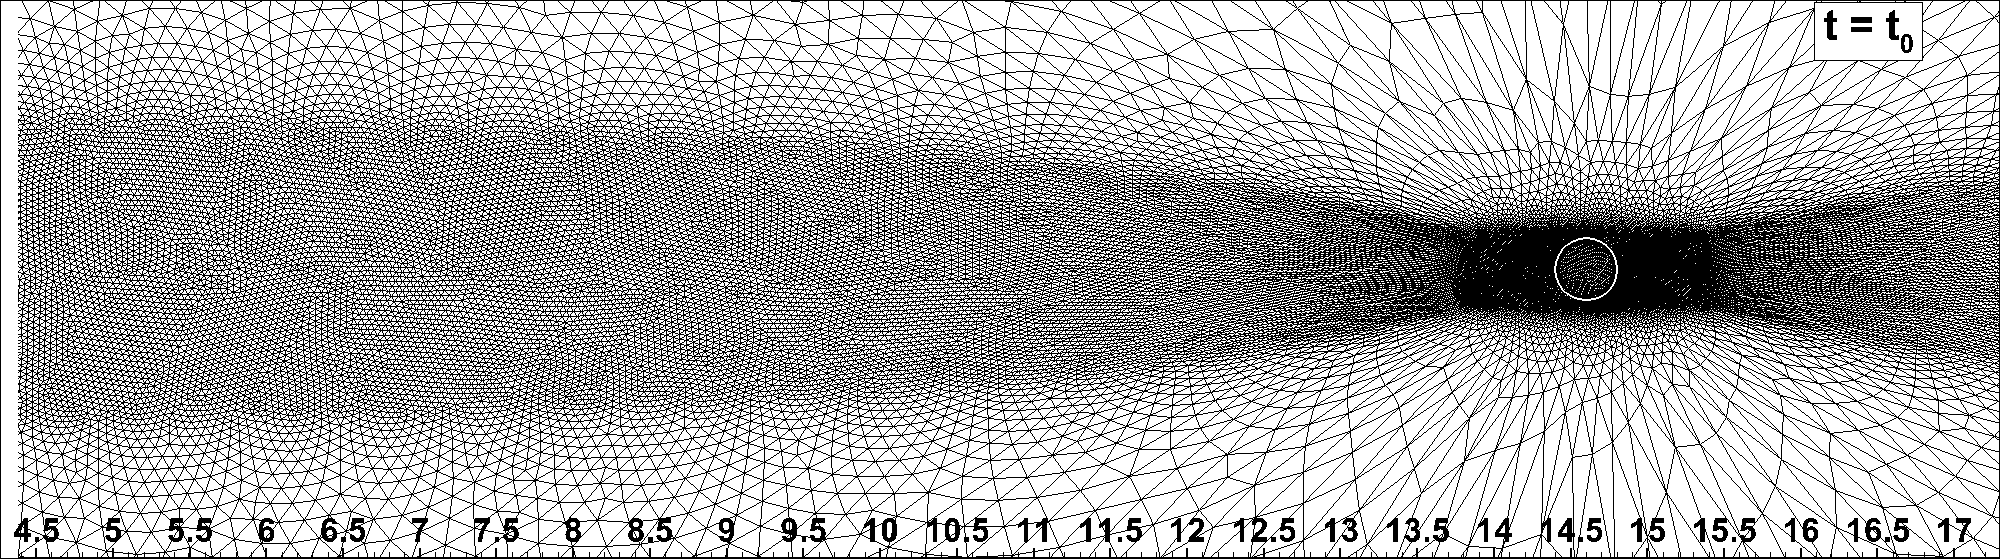
\includegraphics[width=0.9\linewidth]{figure3b}}\\
		\subbottom[три периода $t_0+3T$\label{fig:setka3_mov_c}]{%
			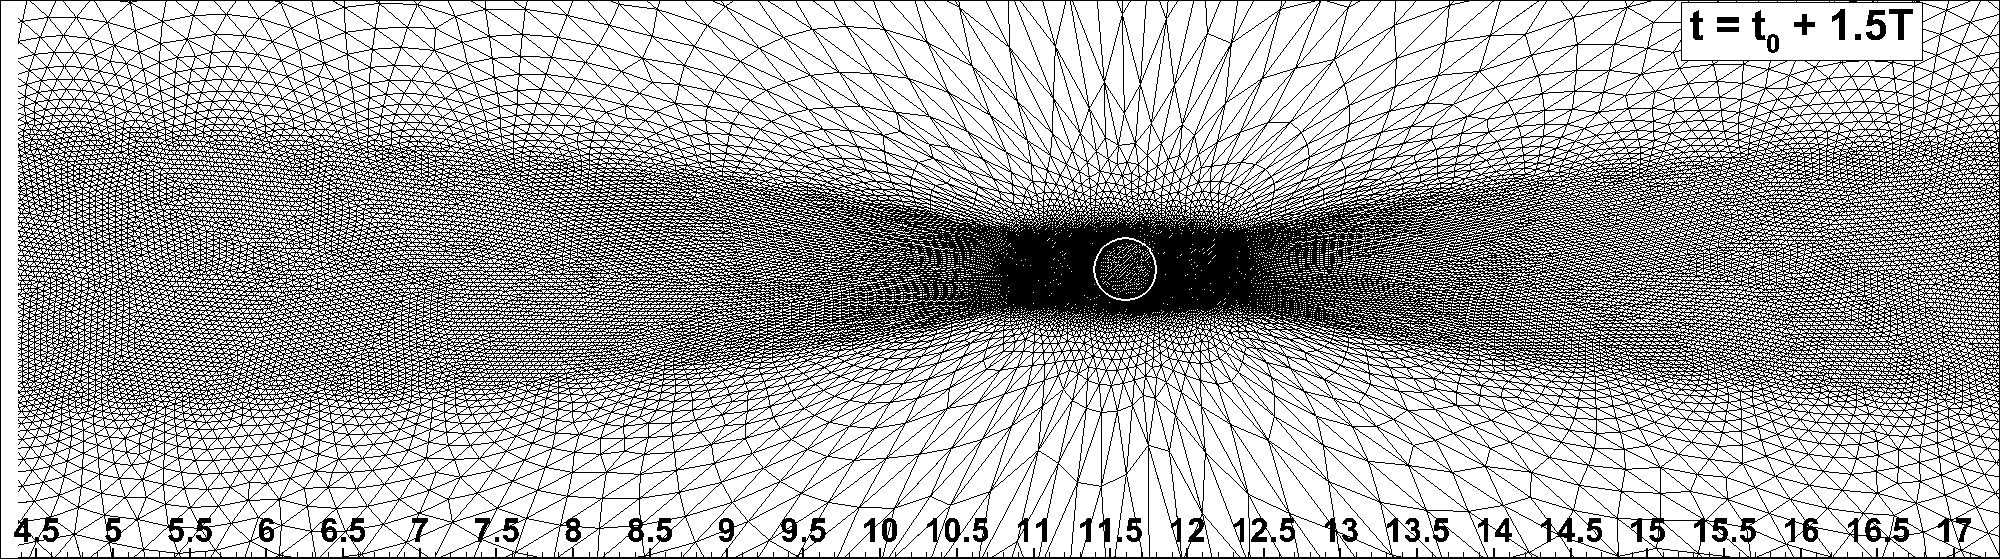
\includegraphics[width=0.9\linewidth]{figure3c}}\\
		\subbottom[четыре с половиной периода $t_0+4.5T$\label{fig:setka3_mov_d}]{%
			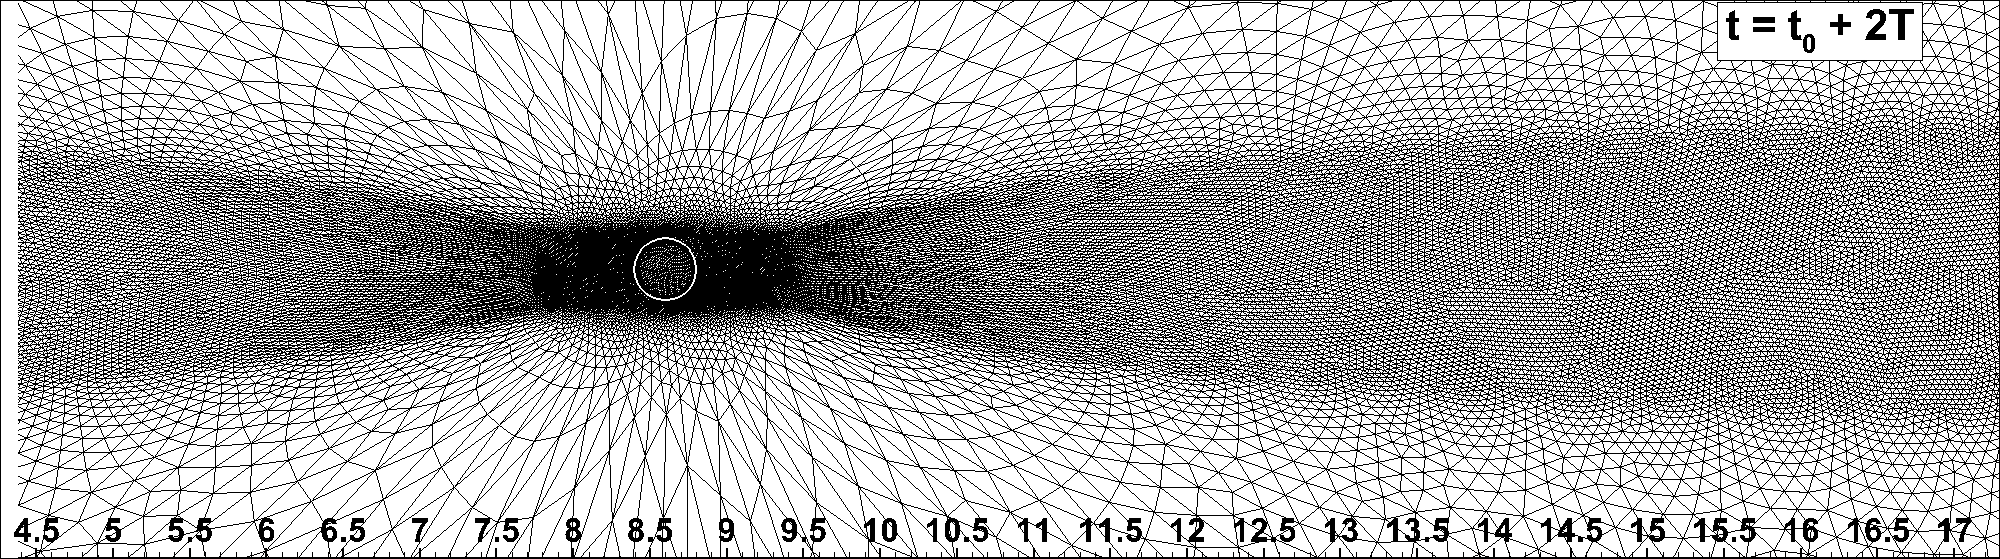
\includegraphics[width=0.9\linewidth]{figure3d}}\\
	}
	\caption[Адаптация сетки 3 с течением времени]{Адаптация сетки 3 с течением времени. а) недеформированная сетка (сетка 2) и её адаптация на три момента времени: б)- начало периода $t_0$ , полтора периода $t_0+1.5T$ и три периода $t_0+3T$.}
	\label{fig:setka3_mov}
\end{figure}
\begin{figure}
	\begin{minipage}{0.45\linewidth}
		\center{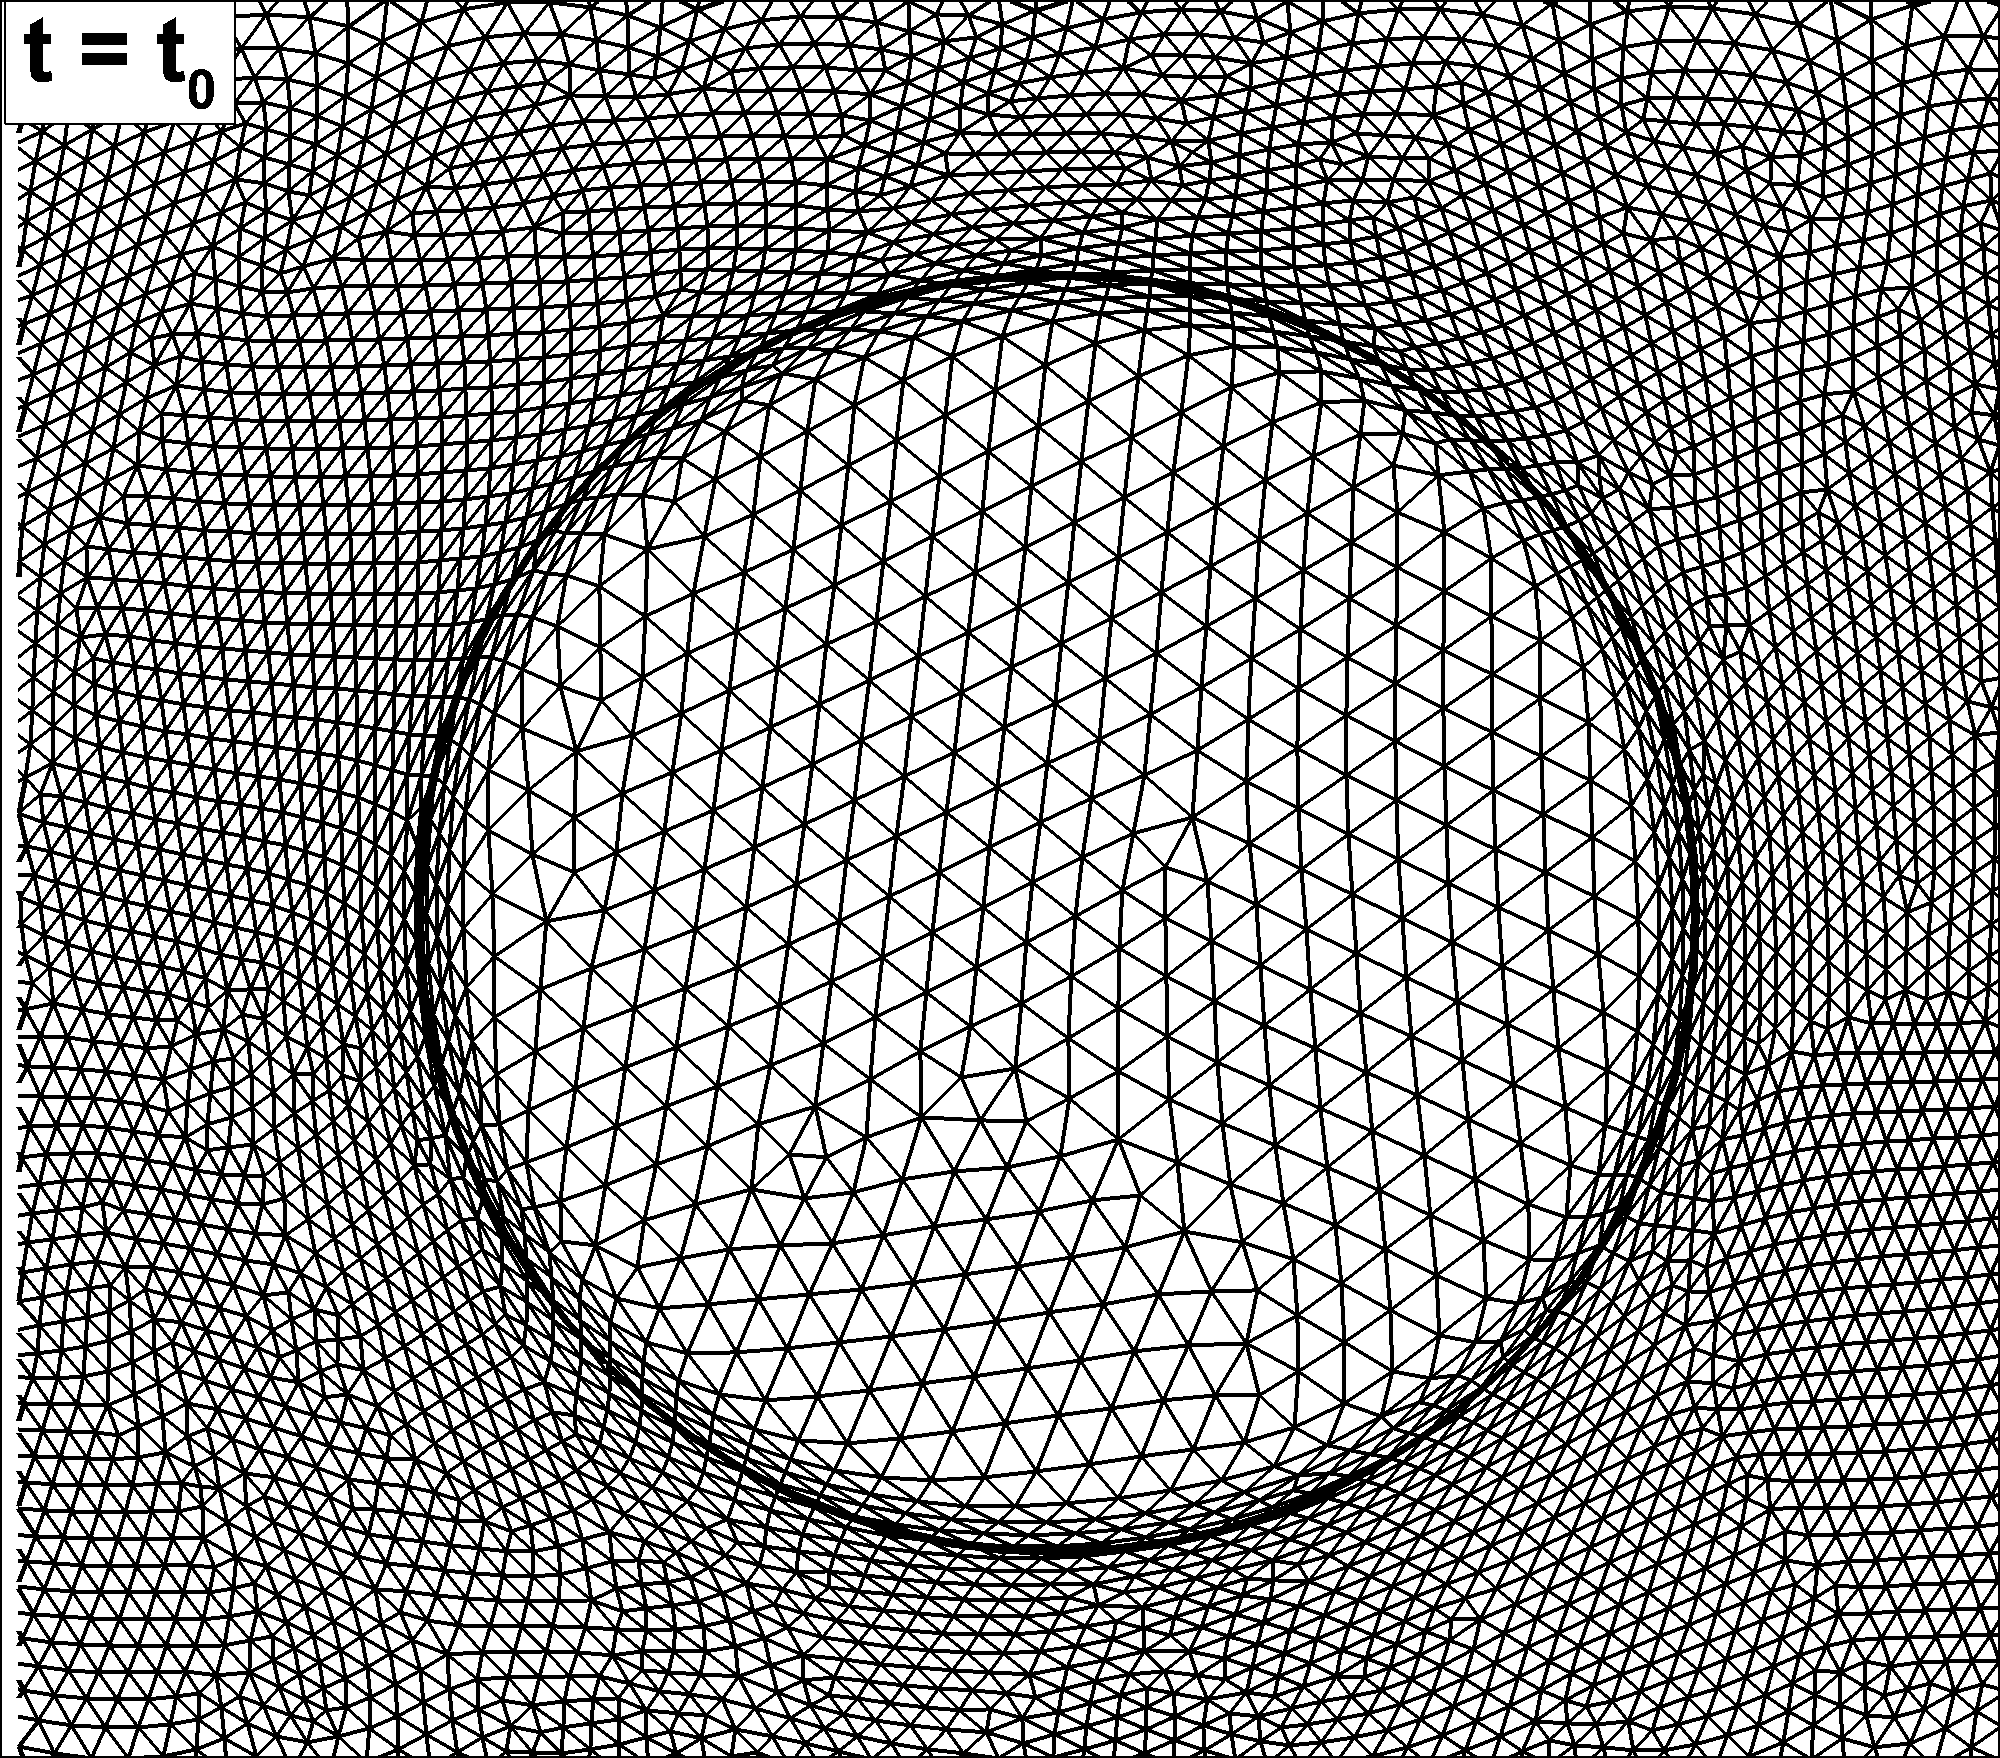
\includegraphics[width=1\linewidth]{figure4a}\\ a) на начало периода $t_0$}
	\end{minipage}
	\hfill
	\begin{minipage}{0.45\linewidth}
		\center{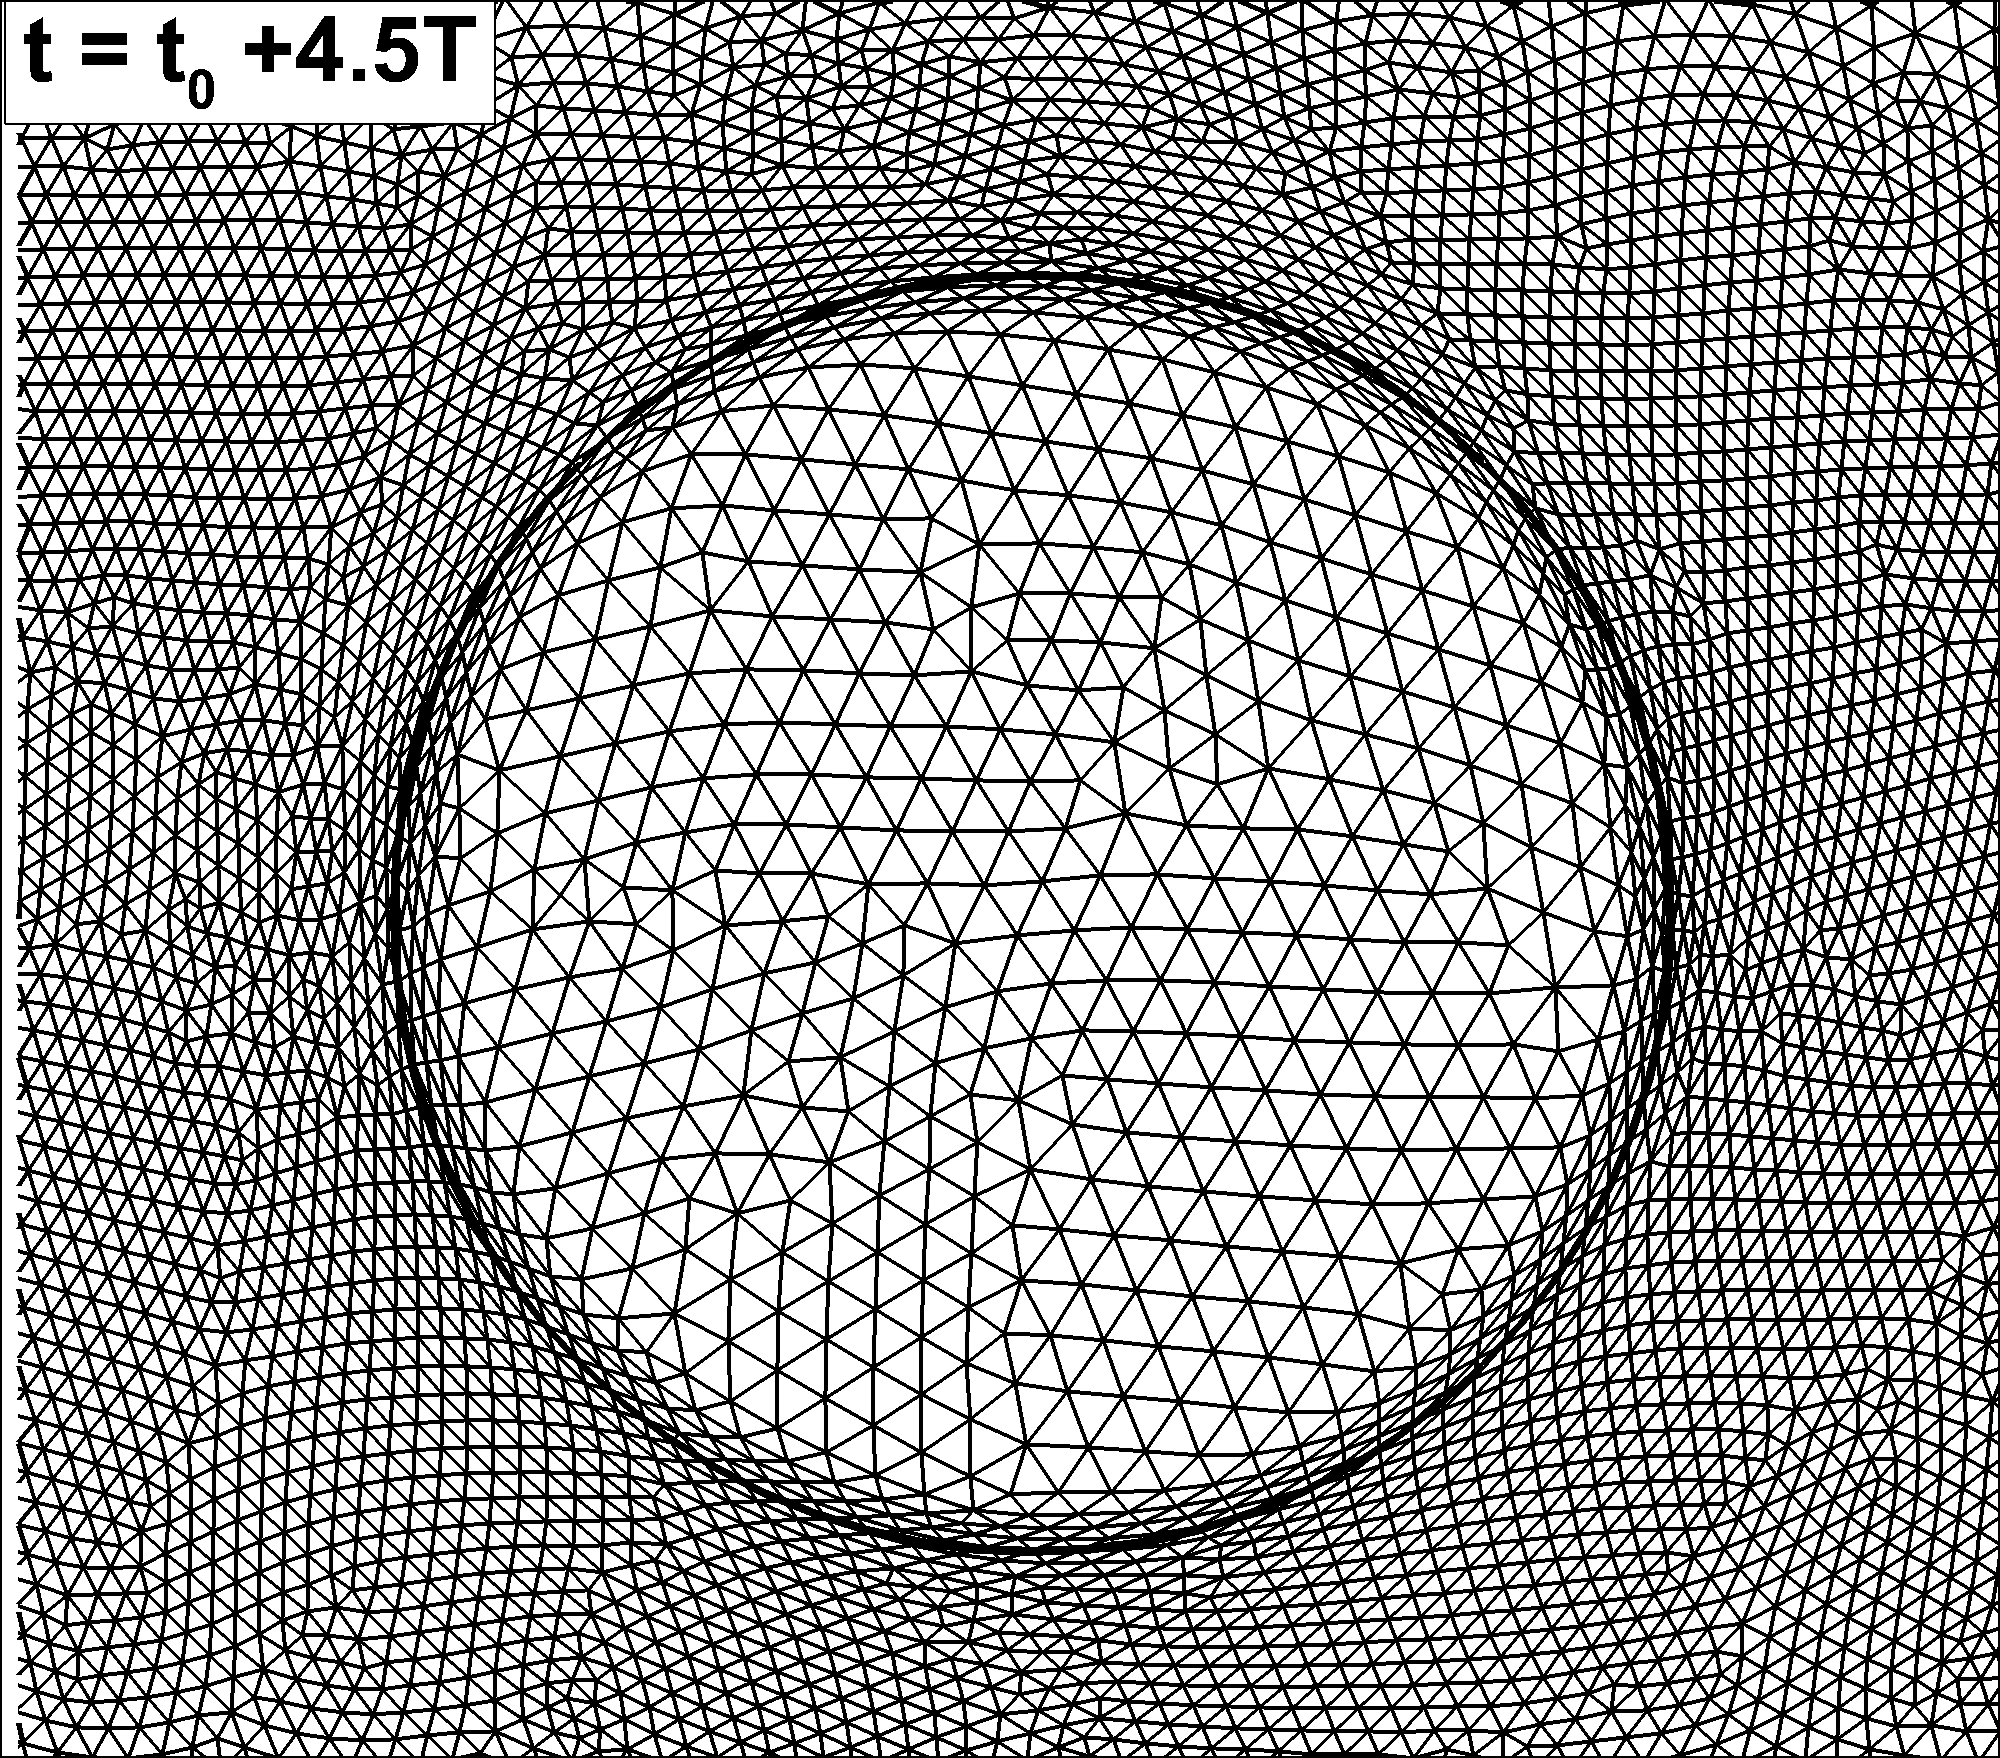
\includegraphics[width=1\linewidth]{figure4b}\\ б) на $t_0+4.5T$}
	\end{minipage} 
	\vspace{10 pt}
	\caption{Сетка вблизи препятствия на начало периода $t_0$ и четыре с половиной периода $t_0+4.5T$ }
	\label{fig:setka3_zoom}
\end{figure}

Закон адаптации сетки определяется управляющей функцией  $\rho(\mathbf{x})$ в уравнении~\eqref{eq:jasak}. Так как обтекаемое тело симметрично, то достаточно определить зависимость управляющей функции только от радиального направления  $r$ с центром, совпадающим с центром цилиндра. Данная функция должна определять сгущение точек с внешней и внутренней стороны границы цилиндра и не изменять исходную сетку при удалении от центра цилиндрического препятствия. Этим условиям удовлетворяют функции типа гауссиана с управляющими параметрами
\begin{equation}\label{eq:gaussian}
\rho{r} = \left\{
\begin{aligned}
&A \exp{\left[-\frac{\ln 2}{b_1}(r - R)^{n_1}\right]+1}, \quad r\le R,\\
&A \exp{\left[-\frac{\ln 2}{b_2}(r - R)^{n_2}\right]+1}, \quad r > R.\\
\end{aligned}
\right.
\end{equation}
Здесь амплитуда  $A$ и чётные показатели степени $n_1, n_2$,   определяют величину сгущения, значения полуширины гауссиана $b_1, b_2$,   задают толщины областей сгущение внутри и вне цилиндра, соответственно. В настоящем расчёте эти параметры полагались равными следующим значениям
\begin{equation}\label{eq:values}
A = 9, \quad n_1 = n_2 = 4, \quad b_1 = 1.6\cdot 10^{-7}, \quad b_2 = 0.1
\end{equation}
Функция~\eqref{eq:gaussian} с параметрами~\eqref{eq:values} трижды непрерывно дифференцируема и её график приведён на рисунке 5.
\begin{figure}[ht]
	\centering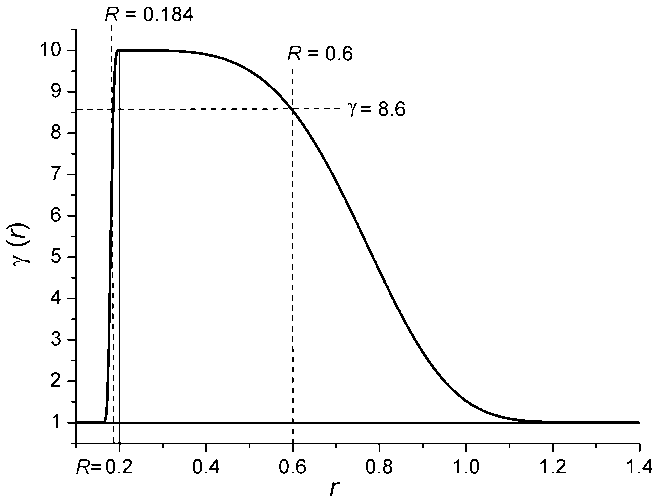
\includegraphics[width=0.45\linewidth]{figure5}
	\caption{График управляющей функции $\rho(r)$}
	\label{fig:monitor_func}
\end{figure}

Из этого графика можно видеть, что наиболее сильная адаптация сетки (уменьшение амплитуды $A$ на 46\%) к границе цилиндра наблюдается на расстоянии приблизительно равным $0.08R$   от границы цилиндра во внутренней области и на расстоянии $3R$ во внешней области. На расстояниях больших $3R$  управляющая функция экспоненциально понижается до единицы, что исключает адаптацию сетки вдали от центра цилиндра в направлении движения цилиндра. Такое изменение сетки можно наблюдать на рисунке 3. Из распределения узлов сетки, показанных на рисунке~\ref{fig:setka3_mov} видно, что в направлении перпендикулярном движению сетка сильно деформируется. Это явление связано с тем, что число узлов в адаптивной сетке не увеличивается, а в направлении перпендикулярном движению исходная недеформированная сетка 2 (на рисунке~\ref{fig:setka3_mov_a}) имеет меньшую плотность распределения узлов.

Из рисунков~\ref{fig:setka3_mov}~и~\ref{fig:setka3_zoom} видно, что адаптация сетки происходит практически однородно и не зависит от положения цилиндра в абсолютной системе координат. То есть фактически можно считать, что деформированная в начальный момент времени сетка перемещается как жёсткая конструкция в направлении движения цилиндра.

Также обратим внимание (см. рисунок \ref{fig:setka3_zoom}), что при использовании изотропной управляющей функции (зависимость только от радиуса) не приводит к сильной деформации элементов сетки в области движения цилиндрического препятствия и сетка вне узкой окрестности вдоль границы цилиндра близка к квазиравномерной.

В процессе адаптации грубой сетки 2 размер элементов сетки в окрестности границы цилиндра имеет размер в среднем в 2.5 раза меньший, чем размер аналогичных элементов подробной сетки 1. Это можно видеть на рисунке~\ref{fig:cell_size}, где показано распределение минимальных высот треугольников на подробной сетке (рисунок~\ref{fig:cell_size_a}) и на грубой сетке после адаптации (рисунок~\ref{fig:cell_size_b}). 
\begin{figure}
	{\centering
		\subbottom[List-of-Figures entry][подробная сетка\label{fig:cell_size_a}]{%
			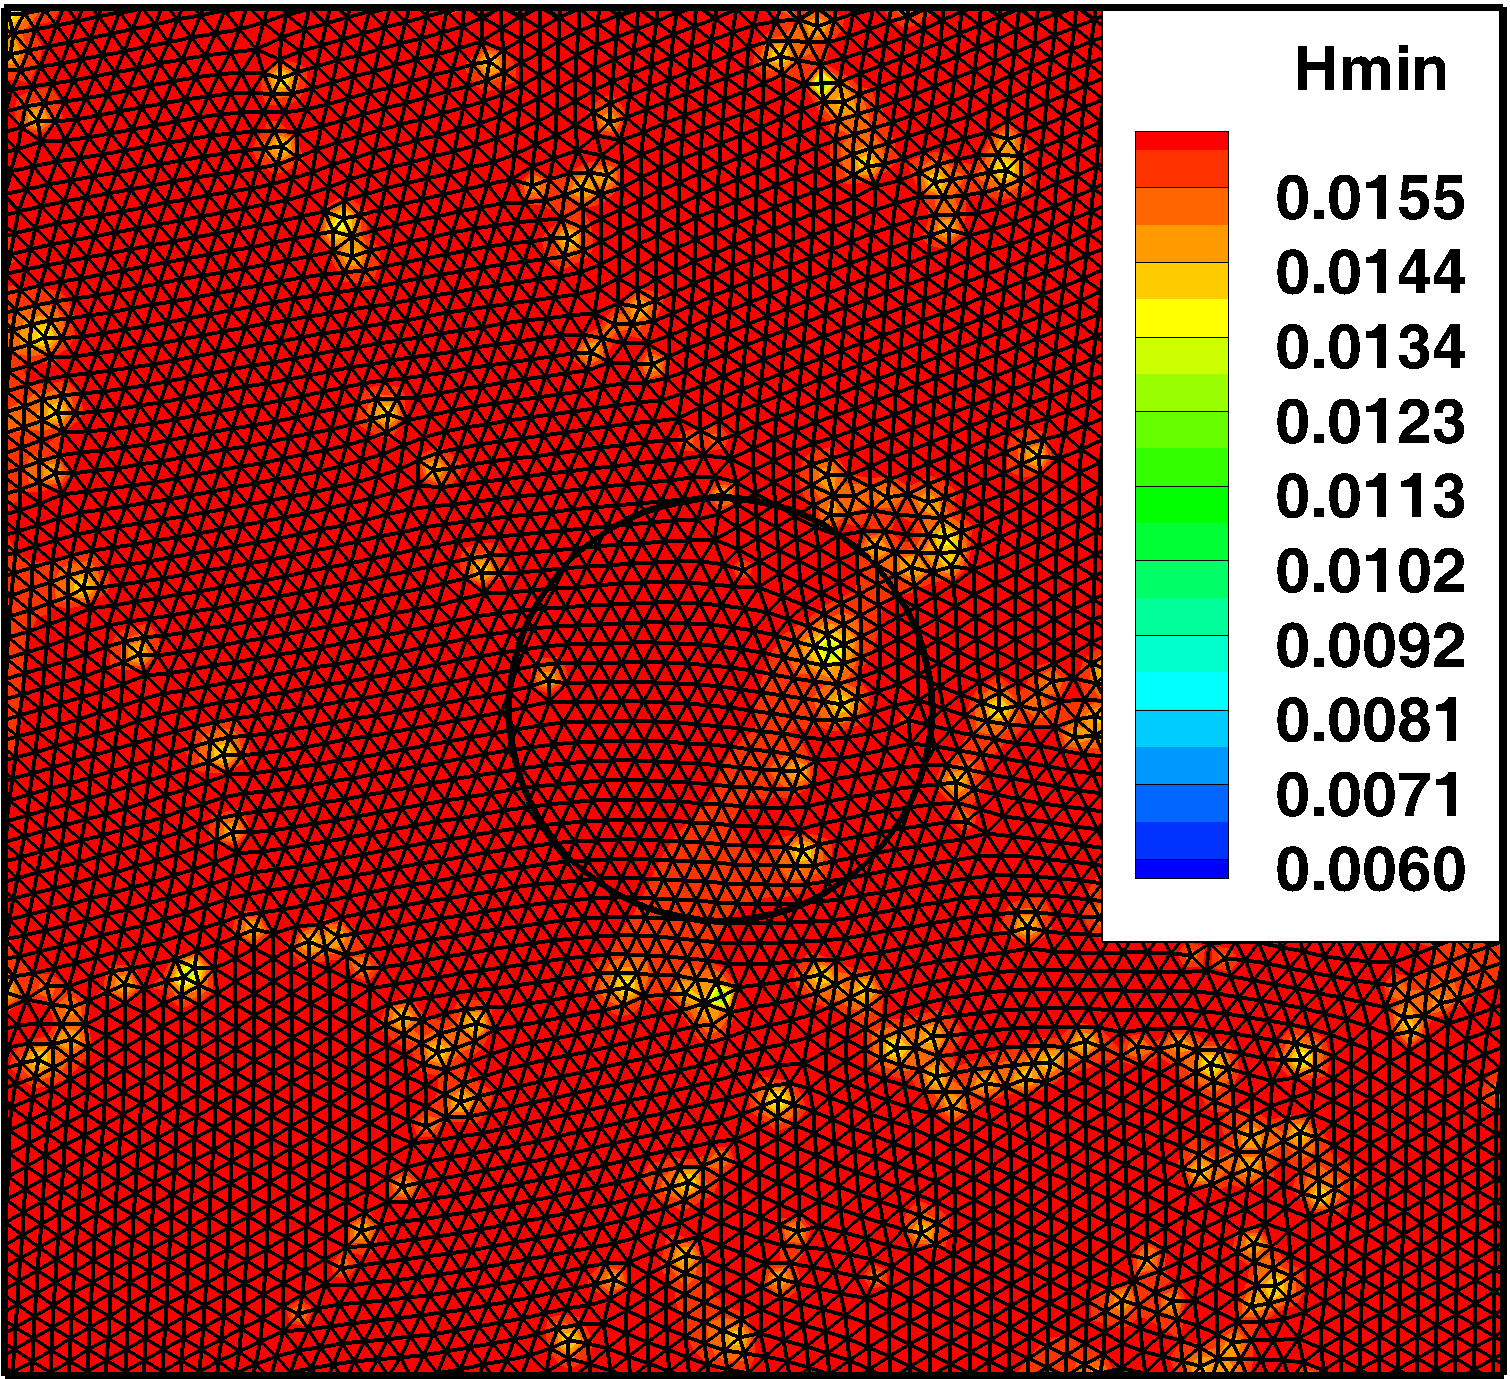
\includegraphics[width=0.45\linewidth]{figure6a}}
		\hfill
		\subbottom[адаптированная грубая сетка\label{fig:cell_size_b}]{%
			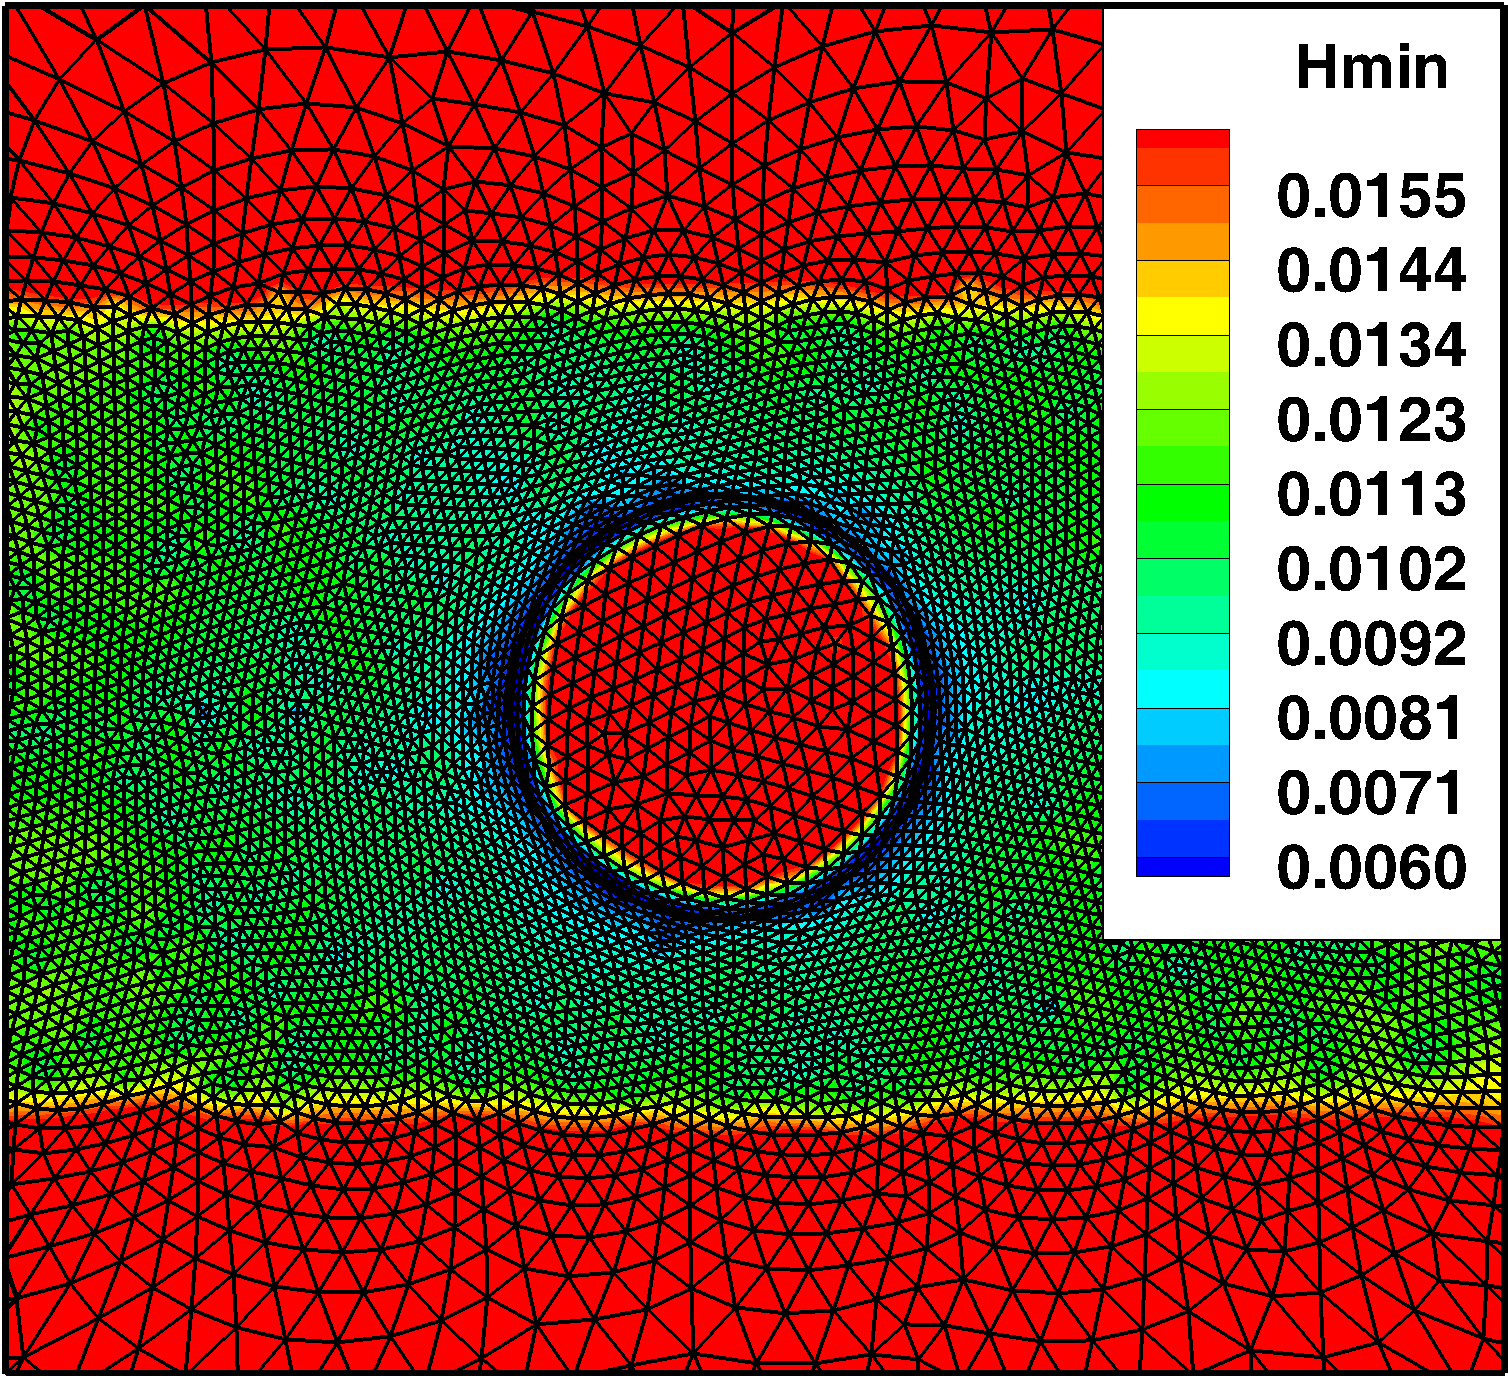
\includegraphics[width=0.45\linewidth]{figure6b}}
	}
	\caption[Пример распределения минимальных высот треугольников в расчётных сетках]{Пример распределения минимальных высот треугольников в расчётных сетках: а) подробная сетка (сетка 1), б) адаптированная грубая сетка (сетка~3)}
	\label{fig:cell_size}
\end{figure}

При выполнении расчётов движущегося цилиндра на всех трёх сетках шаг интегрирования по времени выбирался согласно следующему критерию
\begin{equation}\label{eq:time_step}
\Delta t  =\min(\Delta t_{CFD}, \Delta t_{MOV})
\end{equation}
где   $\Delta t_{CFD}$ – шаг определяемый устойчивостью разностной схемы и обеспечивающий корректность нестационарного интегрирования,   $\Delta t_{MOV}$ – временной шаг, выбираемый из условия прохождения приграничных ячеек границей цилиндра не менее чем за один шаг при расчёте временного слоя  $t_1 = t_0+\Delta t$ 
.\begin{equation}\label{eq:time_step_mov}
\Delta t_{MOV} < \frac{h_{\mathrm{min}}}{|U_B|}.
\end{equation}
Здесь  $h_{\mathrm{min}}$ минимальный размер приграничного элемента сетки на время  $t_0$.
\begin{figure}
	{\centering
		\subbottom[List-of-Figures entry][начало периода $t_0$\label{fig:vorticity_a}]{%
			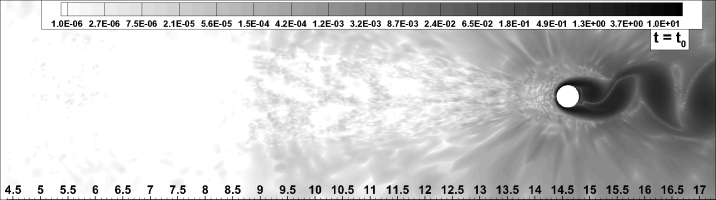
\includegraphics[width=0.9\linewidth]{figure7a}}\\
		\subbottom[полтора периода $t_0+1.5T$\label{fig:vorticity_b}]{%
			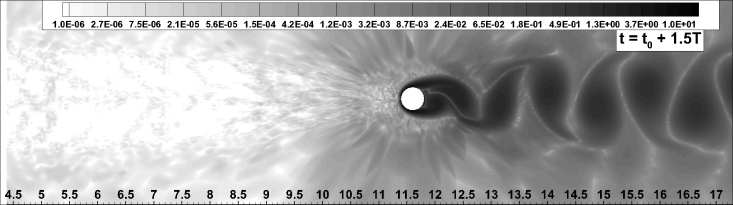
\includegraphics[width=0.9\linewidth]{figure7b}}\\
		\subbottom[три периода $t_0+3T$\label{fig:vorticity_c}]{%
			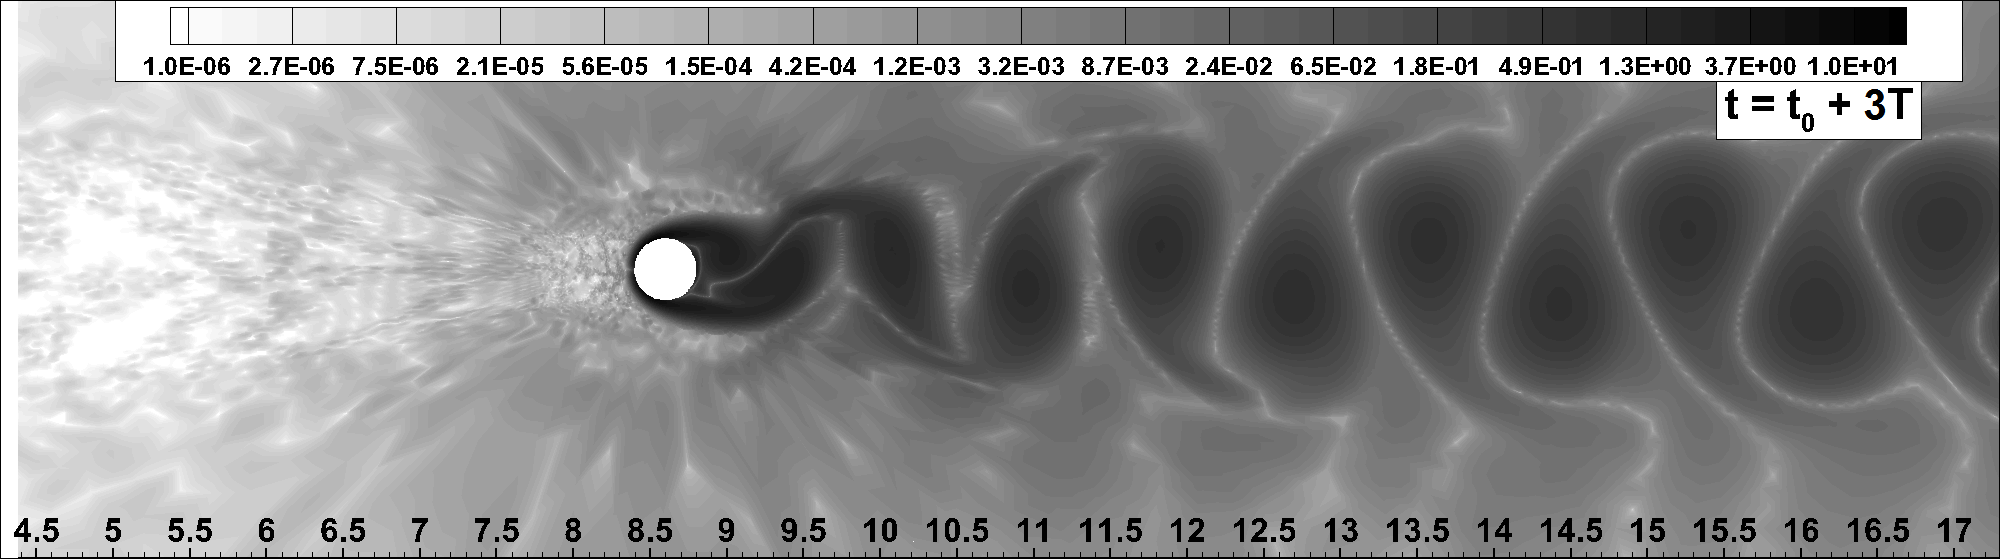
\includegraphics[width=0.9\linewidth]{figure7c}}\\
		\subbottom[четыре с половиной периода $t_0+4.5T$\label{fig:vorticity_d}]{%
			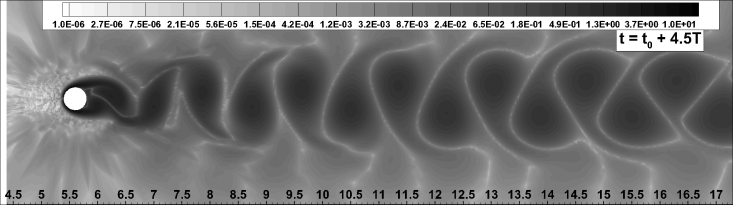
\includegraphics[width=0.9\linewidth]{figure7d}}\\
	}
	\caption[Распределение завихренности на четыре момента времени]{Распределение завихренности на четыре момента времени: а) начало периода $t_0$ , б) полтора периода $t_0+1.5T$ , в) три периода $t_0+3T$ и г) четыре с половиной периода $t_0+4.5T$}
	\label{fig:vorticity}
\end{figure} 

Общая картина течения после выполнения расчёта с использованием адаптивной сетки показана на рисунке~\ref{fig:vorticity}, где приведены поля завихренности на различные моменты времени. В таблице~\ref{tabl:table} приведены средние значение коэффициента сопротивления  и числа Струхаля Sh, полученные по результатам этих расчетов на трёх сетках и экспериментальные значения из работы~\cite{henderson1997nonlinear}. Число Струхаля  Sh определено с помощью преобразования Фурье.
\begin{table}[htbp]
	\centering
	\changecaptionwidth\captionwidth{15cm}
	\caption{Средние значения коэффициентов силы сопротивления и число Струхаля, полученные расчётом на разных сетках.}	\label{tabl:table}%
	\begin{tabular}{|c|c|c|c|c|}
	  \hline
	  \hline
	& Эксперимент~\cite{henderson1997nonlinear} & сетка 1 & сетка 2 & сетка 3 \\ \hline
	Sh               & 0.19        & 0.189   & 0.186   & 0.191   \\ 
	$\overline{C}_d$ & 1.34        & 1.218   & 1.118   & 1.301   \\  \hline
	\hline
	\end{tabular}
\end{table}
\clearpage